\documentclass[tikz,border=3pt]{standalone}
\usepackage{pgfplots}
\pgfplotsset{compat=1.18}

\begin{document}
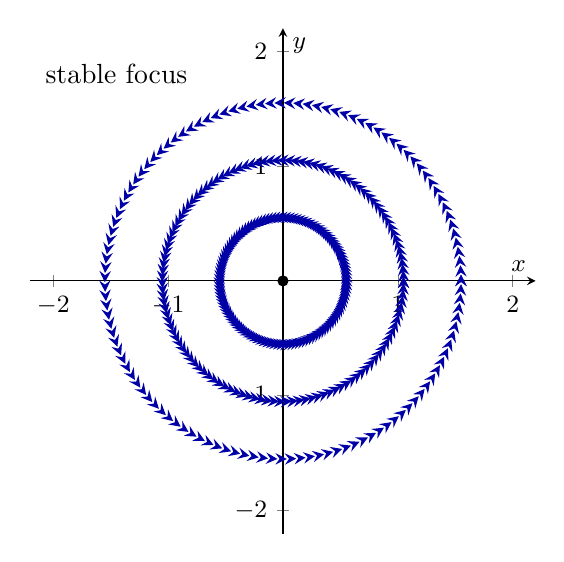
\begin{tikzpicture}
\begin{axis}[
  width=8cm, height=8cm,
  axis lines=middle,
  xlabel={$x$}, ylabel={$y$},
  xmin=-2.2, xmax=2.2, ymin=-2.2, ymax=2.2,
  xtick={-2,-1,1,2}, ytick={-2,-1,1,2},
  tick label style={font=\small},
  label style={font=\small},
  axis equal image,
]
  \foreach \r in {0.55,1.05,1.55} {
    \addplot[blue!65!black, thick, domain=0:360, samples=120,
      quiver={u={-y},v={x},scale arrows=0.035},-stealth]
      ({\r*cos(x)},{\r*sin(x)});
  }
  \addplot[only marks, mark=*, mark size=1.8pt, black] coordinates {(0,0)};
  \node[name=focus,xshift=0pt,yshift=0pt] at (axis cs:-1.45,1.8) {stable focus};
\end{axis}
\end{tikzpicture}
\end{document}
